\chapter{软件系统与操作流程}

密码原语解决具体数学问题，软件系统还要负责组合选择、参数检查、对象保存和用户操作。本章
介绍系统怎样把后端、公共协议和应用入口分开，以及新增HIBE或IBS时需要完成哪些工作。

\section{分层软件架构}

系统自下而上分为基础设施层、密码原语层、组合层、协议层和应用层。基础设施层提供规范编码、
随机源、域分隔哈希、错误处理和状态文件保存。密码原语层分别实现HIBE和IBS。组合层根据配置
选择后端，并在生成密钥前完成能力与容量检查。协议层接入第三章的五个IB-ME算法。最上层提供
命令行、实验工具和浏览器界面。

\begin{figure}[H]
\centering
\begin{tikzpicture}[node distance=7mm and 8mm]
 \node[flow,text width=92mm] (web) {应用层：浏览器、CLI、实验工具};
 \node[flow,below=of web,text width=92mm] (protocol) {协议层：IB-ME五算法、Hybrid、字节认证};
 \node[check,below=of protocol,xshift=-27mm,text width=38mm] (assembly) {组合层\\SuiteConfig、注册表、预检};
 \node[check,below=of protocol,xshift=27mm,text width=38mm] (state) {状态层\\固定发钥、对象保存、恢复};
 \node[flow,below=of assembly,text width=38mm] (hibe) {HIBE后端\\LATTE、Lai};
 \node[flow,below=of state,text width=38mm] (ibs) {IBS后端\\六种签名实现};
 \node[check,below=of protocol,yshift=-48mm,text width=92mm] (core) {基础设施：规范编码、随机源、哈希、错误处理};
 \draw[flowarrow](web)--(protocol);
 \draw[flowarrow](protocol)--(assembly);
 \draw[flowarrow](protocol)--(state);
 \draw[flowarrow](assembly)--(hibe);
 \draw[flowarrow](assembly.south)--++(0,-3mm)-|(ibs.north);
 \draw[flowarrow](hibe)--(core);
 \draw[flowarrow](ibs)--(core);
\end{tikzpicture}
\caption{软件系统的分层结构}
\label{fig:system-structure}
\end{figure}

公共协议通过接口和组合配置调用后端、读取容量和格式。应用层使用统一角色对象与密文字节，同一套页面、状态管理和错误处理服务不同组合。

\section{原语接口的调用关系}
机构建立系统时，分别调用HIBE和IBS的初始化操作，取得两套主公钥与主私钥。为接收者发钥时，
HIBE根据接收身份生成一级密钥；为发送者发钥时，IBS根据发送身份生成签名密钥。
发送消息时，IBS签署协议消息，HIBE加密随机种子；接收消息时，HIBE按认可的发送身份生成叶密钥，
恢复种子，再由IBS检查发送者签名。表~\ref{tab:backend-interfaces}列出各操作的输入与结果。

\begin{table}[H]
\centering\small
\caption{HIBE与IBS的操作及输入输出}
\label{tab:backend-interfaces}
\begin{tabularx}{\textwidth}{@{}p{.19\textwidth}p{.37\textwidth}X@{}}
\toprule
\rowcolor{black!8} 操作 & 主要输入 & 输出与用途 \\
\midrule
HIBE初始化 & HIBE参数与随机源 & HIBE主公钥、主私钥 \\
接收方密钥生成 & HIBE主私钥、接收身份 & 接收者一级密钥 \\
叶密钥委派 & 一级密钥、认可发送身份 & 绑定双方身份的叶密钥 \\
种子加密 & HIBE主公钥、双方身份、随机种子 & 种子密文 \\
种子解密 & 叶密钥、种子密文 & 随机种子或拒绝 \\
\midrule
IBS初始化 & IBS参数与随机源 & IBS主公钥、主私钥 \\
发送方密钥生成 & IBS主私钥、发送身份 & 发送者签名密钥 \\
消息签名 & 发送者密钥、规范协议消息 & 身份基签名 \\
身份验签 & IBS主公钥、发送身份、消息及签名 & 通过或拒绝 \\
\bottomrule
\end{tabularx}
\end{table}

保存对象时，各后端将主公钥、私钥、密文和签名编码为字节；加载时从字节还原对象，并检查版本、
长度、数值范围和身份信息。程序运行使用操作系统随机源，测试可传入固定随机流以复现计算过程。

\section{组合配置与接入流程}

\subsection{组合配置与运行前检查}
一套组合配置需要回答三个问题：采用哪些算法、允许多大的身份和消息、对象按什么格式保存。
系统将这些设置保存在$\mathsf{SuiteConfig}$中，并为其计算配置摘要。主公钥和角色密钥携带该摘要，
导入时据此核对是否来自同一套设置。

\begin{table}[H]
\centering\small
\caption{组合配置的三类设置}
\label{tab:suite-settings}
\begin{tabularx}{\textwidth}{@{}p{.19\textwidth}p{.36\textwidth}X@{}}
\toprule
\rowcolor{black!8} 类别 & 设置内容 & 运行前核对 \\
\midrule
算法与参数 & HIBE、IBS及各自的参数档 & 对应后端可用，HIBE支持两层身份 \\
身份与消息 & 身份长度、种子长度、签名上界及载荷预算 & 双方身份可编码，32字节种子可加密，签名与消息可装入载荷 \\
对象与环境 & 密钥和签名格式、协议版本、所需数学库 & 编码版本一致，所需库及原生组件可用 \\
\bottomrule
\end{tabularx}
\end{table}

程序先完成表中的检查，再生成系统密钥。消息上限由签名输入上限、签名长度和载荷预算共同计算；
配置不足时，界面显示所需长度和当前上限，用户据此调整载荷预算或选择另一组合。

\subsection{新增HIBE或IBS的接入步骤}

接入新HIBE时，实现者完成五个HIBE方法和五类对象，声明两层身份宽度、种子容量和参数预设，
再向注册表提供一个后端描述。接入新IBS时，实现四个密码方法、签名加载和四类对象，声明身份、
签名输入及签名输出上限。新后端可复用公共协议、混合加密、字节认证、状态管理和应用入口。

\begin{figure}[H]
\centering
\begin{tikzpicture}[node distance=7mm and 7mm]
 \node[flow,text width=36mm] (alg) {实现论文算法\\与严格对象};
 \node[flow,right=of alg,text width=36mm] (cap) {声明参数、容量\\和编码格式};
 \node[flow,right=of cap,text width=36mm] (reg) {注册BackendSpec\\获得SuiteConfig};
 \node[check,below=of cap,text width=38mm] (unit) {原语正例、错身份\\篡改与恢复测试};
 \node[check,left=of unit,text width=38mm] (combo) {与现有另一类原语\\完成组合测试};
 \node[check,right=of unit,text width=38mm] (app) {沿用CLI与Web\\完成实际收发};
 \draw[flowarrow](alg)--(cap);
 \draw[flowarrow](cap)--(reg);
 \draw[flowarrow](reg)--(unit);
 \draw[flowarrow](unit)--(combo);
 \draw[flowarrow](unit)--(app);
\end{tikzpicture}
\caption{新增密码后端的接入过程}
\label{fig:new-backend}
\end{figure}

以Wang--PW为例，新增代码位于独立IBS目录，向外暴露与Sageloli、SRGG相同的方法。注册描述声明
目标档$s0$-4、393,320字节签名和4,096字节签名输入上限。组合层据此算出3,924字节应用容量，
并把混合载荷预算提高到能够容纳该签名的范围。随后直接复用LATTE、五个IB-ME算法、命令行角色
导入和错误输入流程；公共协议仍使用统一接口和处理顺序。



\section{固定发钥与持久状态}

发钥机构需要长期保存机构状态，并保证同一身份能够取回
先前发布的密钥。作品为HIBE接收者和IBS发送者分别维护发钥记录。

发钥时，程序先记录待处理身份，再调用底层算法生成密钥。完整的机构状态保存成功后，才向用户
发布密钥。处理中断时，待处理记录保留下来，重启后据此识别尚未完成的发钥操作。

加载状态时，系统按图~\ref{fig:state-recovery}检查组合配置、公开上下文、参数快照、对象类型和
身份绑定。后端随后检查自己的代数关系，例如LATTE叶密钥方程、SRGG对象形状或Wang--PW的
$AX+H_1=G$关系。通过后才恢复运行实例。

\begin{figure}[H]
\centering
\begin{tikzpicture}[node distance=8mm and 8mm]
 \node[flow,text width=34mm] (files) {读取公钥对象\\机构状态与角色密钥};
 \node[flow,right=of files,text width=34mm] (codec) {规范解码\\版本与长度检查};
 \node[flow,right=of codec,text width=34mm] (bind) {配置摘要、身份\\主公钥绑定};
 \node[check,below=of codec,text width=40mm] (math) {后端代数关系与状态账本检查};
 \node[check,left=of math,text width=36mm] (runtime) {恢复运行实例\\继续加密或解密};
 \draw[flowarrow](files)--(codec);
 \draw[flowarrow](codec)--(bind);
 \draw[flowarrow](bind)--(math);
 \draw[flowarrow](math)--(runtime);
\end{tikzpicture}
\caption{持久对象恢复流程}
\label{fig:state-recovery}
\end{figure}

主公钥、发送方密钥、接收方密钥和密文可以分别导出。发送端导入主公钥与发送方密钥，接收端导入
主公钥与接收方密钥；HIBE和IBS主私钥由发钥机构保管。发送与接收可在不同进程或主机上执行，
并使用相同的组合配置与编码。

\section{命令行与浏览器操作}

使用者通过命令行或浏览器完成以下流程：
\begin{enumerate}
 \item 选择组合，建立系统，保存机构状态与系统主公钥。
 \item 为发送者Alice和接收者Bob生成密钥，并向双方分发各自的角色对象。
 \item Alice输入Bob的身份和消息，程序完成签名、种子加密与载荷加密，输出密文字节。
 \item Bob导入密文，填写认可的发送者Alice，程序完成身份匹配和签名检查后显示原文。
 \item 再次使用时，命令行加载已保存的主公钥与角色密钥，继续处理消息。
\end{enumerate}
浏览器显示建立、发钥、签名、加密和解密的处理进度，并给出密文长度、实际耗时与结果。
耗时较长的操作由服务端执行；刷新页面后，浏览器可重新连接当前任务。

\begin{figure}[H]
\centering
\includegraphics[width=.98\textwidth]{../../deliveries/2026-10-20-web-redesign/desktop.png}
\caption{消息发送与匹配解密界面}
\label{fig:web-demo}
\end{figure}

图~\ref{fig:web-demo}记录A组的一次实际操作：Alice向Bob发送36字节UTF-8消息，Bob选择Alice为
期望发送者后恢复原文。A、B还分别在同一条密文上执行三种身份错配、翻转1 bit和截短1字节，
均得到拒绝。两组该次密文长度分别为142,095字节和149,255字节。

\begin{figure}[H]
\centering
\begin{minipage}[t]{.49\textwidth}
\centering
\includegraphics[width=\linewidth,trim=420 320 130 180,clip]{../../deliveries/2026-10-20-web-redesign/desktop.png}
\par\smallskip\textbf{（a）身份匹配并恢复原文}
\end{minipage}\hfill
\begin{minipage}[t]{.49\textwidth}
\centering
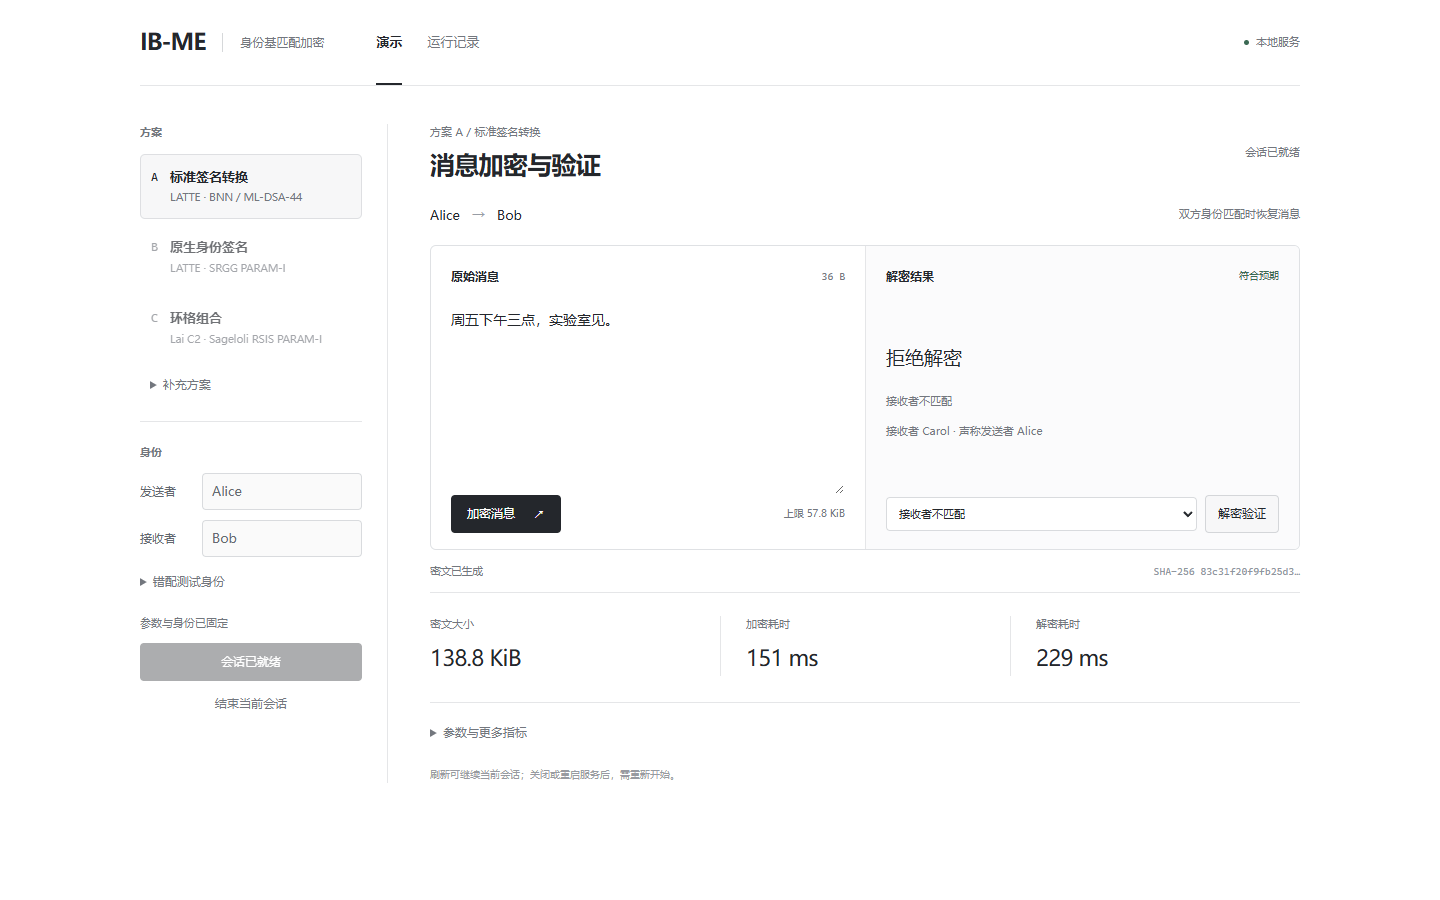
\includegraphics[width=\linewidth,trim=420 320 130 180,clip]{../../deliveries/2026-10-20-web-rejection-screenshots/wrong-receiver.png}
\par\smallskip\textbf{（b）接收身份不匹配并拒绝}
\end{minipage}
\caption{身份匹配与错配结果}
\label{fig:web-demo-details}
\end{figure}

\section{运行优化与部署方式}

除了第五章的三项主要优化，系统还减少两类重复工作。BNN签名包含机构证书和用户消息签名。对
同一身份的连续消息，系统缓存“证书已经验证”的公开结果，但每条消息仍重新验证用户签名。
缓存绑定完整证书、用户公钥和身份，并使用有界LRU管理。

SRGG签名的一部分数值准备只取决于固定签名密钥和数值选项。实现可以复用该计划，每条签名仍
重新生成随机量。实验表明这两类局部缓存对完整流程的影响小于结构化采样、紧凑编码和Lai会话，
系统分别提供证书验证缓存和签名准备复用选项。

系统支持集中部署和分角色部署。集中部署将发钥、发送、接收和浏览器服务放在同一台主机，
由机构统一管理。分角色部署时，发钥机构生成角色对象，发送端与接收端分别导入自己的密钥，
通过文件服务或消息队列交换密文。

\begin{figure}[H]
\centering
\begin{tikzpicture}[node distance=9mm and 12mm]
 \node[check,text width=38mm] (issuer) {发钥机构\\建立系统、签发角色密钥};
 \node[flow,below left=of issuer,text width=36mm] (sender) {发送端\\导入公钥对象与发送方密钥};
 \node[flow,below right=of issuer,text width=36mm] (receiver) {接收端\\导入公钥对象与接收方密钥};
 \node[check,below=of issuer,yshift=-34mm,text width=38mm] (channel) {公开传输通道\\只传递规范密文};
 \draw[flowarrow](issuer)--node[left,font=\small]{发送角色对象}(sender);
 \draw[flowarrow](issuer)--node[right,font=\small]{接收角色对象}(receiver);
 \draw[flowarrow](sender)--(channel);
 \draw[flowarrow](channel)--(receiver);
\end{tikzpicture}
\caption{发钥机构、发送端与接收端的部署关系}
\label{fig:deployment}
\end{figure}



\begin{table}[H]
\centering\small
\caption{安装环境与运行结果}
\label{tab:installation-reproduction}
\begin{tabularx}{\textwidth}{@{}p{.24\textwidth}X@{}}
\toprule
\rowcolor{black!8} 项目 & 环境或结果 \\
\midrule
运行环境 & Xeon Silver 4216；NixOS；Sage~10.9；Python~3.14.7 \\
A、B组合 & 各完成25条操作，覆盖安装、角色对象、消息收发与恢复 \\
C组合 & 完成匹配解密、内部签名拒绝和对象恢复 \\
\bottomrule
\end{tabularx}
\end{table}

\section{本章小结}

软件系统通过稳定接口、组合配置和注册表把底层算法与公共协议分开。新增后端只实现自身算法、
对象与能力声明，随后即可复用五个IB-ME算法、状态管理、CLI和浏览器入口。固定发钥和规范恢复
使系统能够跨进程长期使用，集中部署与分角色部署支持机构内服务和跨主机通信。
